Rozdział przedstawia środowisko ewaluacyjne (ang.\ \textit{framework}) zbudowane na potrzeby
niniejszej pracy. Jego zadaniem jest zestawianie ze sobą konfiguracji przetwarzania zapytania
głosowego, od transkrypcji po wyszukiwanie, w warunkach, w których jedyną różnicą między
porównywanymi przebiegami jest badany czynnik. Opisano kolejno model danych, algebrę węzłów,
budowę i wykonanie grafu oraz sposób zestawiania wyników. Na koniec przedstawiono ścieżkę
wyszukiwania zestawioną z opisanych węzłów oraz interfejs, przez który system jest obsługiwany.
Podrozdział~\ref{sec:eksperymenty} przedstawia pomiary wykonane na tak zbudowanym systemie.

Do ewaluacji wyszukiwania istnieją ustalone narzędzia. Zbiory porównawcze wraz z referencyjnymi
implementacjami metryk rankingowych oceniają listę wyników wobec dokumentów istotnych
\cite{manning2008introduction, lin2020, thakur2021beir}. Nowsze zestawy oceniają jakość
generacji wspomaganej wyszukiwaniem, również w medycynie \cite{pubmed, es2024ragas}. Żadne ze znanych
autorom narzędzi nie obejmuje jednak całej ścieżki od nagrania do rankingu ani nie porównuje
wariantów przetwarzania na tych samych elementach z różnicami liczonymi parami. Opisane środowisko
uzupełnia te braki, korzystając z istniejących implementacji metryk tam, gdzie one wystarczają.

\section{Opis systemu}
\label{sec:opis}
Zasadniczą zaletą środowiska jest izolacja badanego czynnika: porównywane warianty przetwarzają
w jednym przebiegu ten sam sygnał i ten sam korpus, więc różnica wyników ma dokładnie jedno
źródło. Każdy przebieg jest odtwarzalny z zapisanej konfiguracji, a dołożenie kolejnego wariantu
sprowadza się do zmiany kilku węzłów grafu, bez modyfikacji pozostałych.

\subsection{Przegląd systemu}
\label{sec:przeglad-systemu}
System sprowadza pojedynczy
eksperyment do jednego grafu, przez który przepływają nazwane wartości, a jego budowa jest zawsze
taka sama, niezależnie od tego, czy mierzona jest jakość transkrypcji, wyszukiwania czy generowanej
odpowiedzi. Schemat tego przepływu przedstawiono na rysunku~\ref{fig:przegladSystemu}.

\begin{figure}[htbp]
    \centering
    \adjustbox{max width=\linewidth}{\begin{tikzpicture}[
    scale=0.6,
    transform shape,
    font=\small,
    block/.style={
        draw,
        rounded corners=2pt,
        thick,
        minimum width=3.1cm,
        minimum height=1.05cm,
        align=center
    },
    src/.style={block, fill=gray!12},
    trans/.style={block, fill=blue!20},
    met/.style={block, fill=red!12},
    agg/.style={block, fill=orange!25},
    sink/.style={block, fill=green!15},
    arrow/.style={-{Stealth[]}, thick},
    art/.style={font=\scriptsize\itshape, text=gray!60!black, align=center}
]

% ============================================================
% GLOWNY PRZEPLYW
% ============================================================
\node[src]   (zrodlo) at ( 0.0, 0) {Źródła danych\\[-2pt]\scriptsize{typowane pola}};
\node[trans] (przeksz) at ( 6.2, 0) {Węzły\\[-2pt]przekształceń};
\node[met]   (metryki) at (12.4, 0) {Węzły metryk};
\node[agg]   (agreg)   at (18.2, 0) {Agregacja};
\node[sink]  (raport)  at (23.6, 0) {Raport};

\draw[arrow] (zrodlo)  -- node[art, above] {artefakty} (przeksz);
\draw[arrow] (przeksz) -- node[art, above] {artefakty} (metryki);
\draw[arrow] (metryki) -- node[art, above] {wyniki\\elementowe} (agreg);
\draw[arrow] (agreg)   -- (raport);

% ============================================================
% CO KRYJE SIE POD WEZLAMI PRZEKSZTALCEN
% ============================================================
\node[align=center, font=\scriptsize, text=gray!60!black, below=1.05cm of przeksz]
    (opis) {transkrypcja, synteza mowy, embedding,\\
            indeksowanie, wyszukiwanie, zawężanie,\\
            augmentacja, generacja odpowiedzi};
\draw[gray, dashed] (przeksz.south) -- (opis.north);

\node[align=center, font=\scriptsize, text=gray!60!black, below=1.05cm of metryki]
    (opism) {dostawiane automatycznie wszędzie,\\gdzie ich wejścia są obecne};
\draw[gray, dashed] (metryki.south) -- (opism.north);

% ============================================================
% TABLICA ARTEFAKTOW JAKO WSPOLNE PODLOZE
% ============================================================
\node[draw=gray, dashed, rounded corners=4pt, inner sep=0.42cm,
      fit=(zrodlo)(przeksz)(metryki)(agreg)(raport),
      label={[font=\scriptsize\itshape, gray]above:wspólna tablica artefaktów przebiegu}] {};

\end{tikzpicture}
}
    \caption{Przepływ pojedynczego przebiegu. Źródła danych udostępniają typowane pola, węzły
    przekształceń przetwarzają je na kolejne artefakty, węzły metryk odczytują artefakty i zwracają
    wyniki elementowe, a agregacja redukuje je do raportu. Wszystkie węzły wymieniają dane wyłącznie
    przez wspólną tablicę artefaktów przebiegu, nigdy bezpośrednio między sobą.}
    \label{fig:przegladSystemu}
\end{figure}

Przepływ ma cztery etapy. Źródło danych udostępnia typowane pola, takie jak nagranie zapytania,
tekst pytania czy korpus dokumentów. Węzły przekształceń zamieniają je na kolejne artefakty:
transkrybują mowę, embeddują tekst w przestrzeni wektorowej, budują indeks, wyszukują dokumenty,
zawężają ranking albo generują odpowiedź. Węzły metryk odczytują powstałe artefakty, niczego nie
zmieniając, i zwracają wyniki dla poszczególnych elementów. Węzeł agregujący sprowadza je do
raportu, który utrwalają węzły zapisu. O tym, który węzeł czyta od którego, rozstrzygają
krawędzie grafu.

Tabela~\ref{tab:wezly} zestawia dostępne kategorie węzłów wraz z rodzajem modelu, z którego
korzystają. Jest to pełny katalog operacji, z których składa się dowolny eksperyment opisany
w dalszej części rozdziału.

\begin{table}[htbp]
\centering
\small
\begin{tabular}{@{}L{3.3cm}L{7.4cm}L{3.1cm}@{}}
\toprule
\textbf{Kategoria} & \textbf{Węzły (rola)} & \textbf{Model} \\
\midrule
Przygotowanie zapytania & transkrypcja mowy, synteza mowy, optymalizacja, przeredagowanie i korekcja zapytania & ASR, TTS, LLM, korektor \\
Reprezentacja wektorowa & embedding tekstu i audio, fuzja embeddingów, indeksowanie korpusu & modele embeddingowe \\
% Wyszukiwanie & wyszukiwanie (gęste/rzadkie/hybrydowe), przestawianie, MMR, próg & ---, model przestawiający \\
Wyszukiwanie & wyszukiwanie gęste w przestrzeni wektorowej & --- \\
% Augmentacja & zaburzanie audio lub tekstu (z zachowaniem typu) & --- \\
Augmentacja & zaburzanie audio (z zachowaniem typu) & --- \\
Generacja odpowiedzi & odpowiedź z pobranego kontekstu (RAG) & LLM \\
Ewaluacja i zapis & metryki, agregacja, utrwalanie raportu & --- \\
\bottomrule
\end{tabular}
\caption{Kategorie węzłów i wykorzystywane modele. Myślnik oznacza węzły bezmodelowe,
wykonujące operacje na artefaktach bez użycia modelu.}
\label{tab:wezly}
\end{table}

\subsection{Założenia projektowe}
Porównanie wariantów przetwarzania na wspólnych danych wymaga jednorodnych warunków.
Zaprojektowano zatem środowisko, w którym
eksperyment jest \textit{skierowanym grafem acyklicznym} (ang.\ \textit{directed acyclic graph},
DAG). Typowane źródła danych dostarczają wartości pośrednie, a węzły je przekształcają. Każda
wartość przekazywana między węzłami jest nazwanym artefaktem o określonym typie i modalności, jak
nagranie zapytania albo jego embedding. Węzły nie wywołują się nawzajem, lecz wymieniają
je przez wspólną tablicę artefaktów przebiegu. Węzeł deklaruje, jakie artefakty pobiera i
jakie wytwarza, a jego tożsamość jest oddzielona od typu, więc ten sam typ może wystąpić w grafie
wielokrotnie. Krawędzie stanowią część specyfikacji: każda z nich nazywa węzeł i artefakt
źródłowy oraz węzeł i wejście docelowe.

Metryki i agregacja także są węzłami, dzięki czemu każdą metrykę można niezależnie włączyć i
skierować na wybraną gałąź, czyli na wariant przetwarzania odchodzący od wspólnej początkowej
części grafu. Cały eksperyment opisany jest konfiguracją, którą wykonuje wspólny rdzeń, ten sam
dla wiersza poleceń, interfejsu webowego oraz API. Konfiguracja nie
zawiera niczego poza listą węzłów i krawędzi wraz z ich parametrami, więc to graf steruje budową
potoku oraz zachowaniem procedur.

\subsection{Źródła danych i typowane pola}
Źródło danych to zbiór rekordów o typowanych polach, które stają się artefaktami wejściowymi
grafu. Modelowanie polami, zamiast sztywnym schematem, uogólnia działanie systemu na różne modalności
i ścieżki przetwarzania. W definicji zbioru określa się mapowanie kolumn na artefakty, a węzeł
źródłowy udostępnia dokładnie zdefiniowany zestaw kolumn.

Strukturę zbioru opisują relacje między polami, wiążące zapytanie z odpowiedzią referencyjną, z
dokumentami istotnymi wraz z oceną istotności oraz z transkrypcją referencyjną. Dwie referencje
pozostają rozdzielone: tekst pytania jest referencją dla etapu wyszukiwania, a transkrypcja
wypowiedzi referencją jakości ASR.

Zbiór nie narzuca trybu ewaluacji, lecz publikuje zestaw typowanych pól: nagranie zapytania,
tekst pytania, korpus dokumentów, oceny istotności, odpowiedź referencyjną albo transkrypcję
referencyjną. To, co faktycznie jest mierzone, wynika z konfiguracji grafu, czyli z tego, które
węzły przetwarzania i metryk podłączono do udostępnionych pól. Ten sam zbiór obsługuje więc wiele
pomiarów: gdy metryki sięgają po transkrypcję referencyjną, przedmiotem oceny jest jakość ASR, a
gdy po listę wyników i oceny istotności, jakość wyszukiwania. Zadeklarowane właściwości zbioru,
takie jak wymagana modalność i dostępne pola, nie wybierają pomiaru, lecz ograniczają zbiór
poprawnych grafów. Konfiguracja żądająca artefaktu, którego zbiór nie publikuje, zostaje odrzucona
na etapie walidacji. Te same właściwości podpowiadają domyślny dobór metryk, który pozostaje
nadpisywalny. Obsługiwane zbiory obejmują m.in.\ FLEURS \cite{fleurs}, ADMEDVoice
\cite{ADMEDVoice} oraz PubMedQA \cite{jin2019pubmedqa}. Zbiór tekstowy wspierający generowanie poszerza
zestaw publikowanych pól o ścieżkę audio zapytań syntezowaną w czasie wykonania, dzięki czemu
dopuszcza również grafy głosowe. Dokumenty korpusu pozostają tekstem.

Jeden graf może łączyć wiele źródeł, na przykład pytania głosowe z jednego zbioru i korpus
dokumentów z drugiego. Decyduje o tym konfiguracja, która przypisuje każdemu węzłowi źródła rolę
korpusu, pytań albo obu naraz. Oba źródła spina wspólna przestrzeń identyfikatorów: oceny
istotności odwołują się do dokumentów korpusu po identyfikatorze. Zgodność tych przestrzeni jest
sprawdzana przed przebiegiem. Gdy okazują się rozłączne, żaden dokument istotny nie występuje w
korpusie, więc metryki wyszukiwania zostają wyłączone wraz z ostrzeżeniem. Zapobiega to zeru
nieodróżnialnemu od realnie zerowej skuteczności. Metryki niezależne od tego powiązania, jak ocena
odpowiedzi, liczą się dalej.

\subsection{Tablica artefaktów}
Na tablicy artefaktów przebiegu każdy artefakt zajmuje osobne miejsce, adresowane parą: węzeł
wytwarzający (producent) i nazwa artefaktu. Węzeł odczytujący (konsument) nie sięga po artefakt po
samej nazwie, lecz przez powiązanie ustalone przy budowie grafu, wskazujące producenta.
Dzięki temu dwa węzły mogą opublikować artefakt tego samego typu bez kolizji, a przekształcenia
takie jak korekcja, optymalizacja i przeredagowanie publikują osobne artefakty. Do jednego
wejścia może prowadzić kilka krawędzi. Węzeł łączący, jak fuzja wektorów czy scalenie korpusów,
czyta je wszystkie naraz. Węzeł oczekujący jednej wartości deklaruje listę dopuszczalnych
wariantów artefaktu w porządku priorytetu, od najpóźniejszego etapu przetwarzania, i czyta
pierwszy opublikowany. Dla tekstu zapytania lista ta obejmuje kolejno przeredagowanie,
optymalizację, augmentację, korekcję i surową transkrypcję. Nieprzetworzona hipoteza ASR pozostaje
dzięki temu niezmienna, więc WER i CER oblicza się wprost na niej.
Tabela~\ref{tab:artefakty} zestawia artefakty systemu.

\begin{table}[htbp]
\centering
\small
\begin{tabular}{@{}L{3.2cm}L{6.0cm}L{4.6cm}@{}}
\toprule
\textbf{Typ danych} & \textbf{Co obejmuje} & \textbf{Źródło (węzeł)} \\
\midrule
Tekst        & zapytanie, transkrypcja referencyjna, tekst referencyjny pytania, odpowiedzi referencyjne, wygenerowana odpowiedź & źródło danych, transkrypcja, korekcja, optymalizacja i przeredagowanie zapytania, generacja odpowiedzi \\
Audio        & nagranie zapytania                              & źródło danych, synteza mowy \\
Wektor i indeks & embedding zapytania, embedding korpusu, indeks korpusu & embedding, fuzja, indeksowanie korpusu \\
Dokumenty i wyniki & korpus, dokumenty istotne, lista wyników  & źródło danych, wyszukiwanie \\
Wyniki ewaluacji & wyniki elementowe, raport                    & metryki, agregacja \\
\bottomrule
\end{tabular}
\caption{Wspierane typy danych i węzły, które je wytwarzają.}
\label{tab:artefakty}
\end{table}

\subsubsection{Tożsamość elementów}
Każda wartość elementowa jest związana ze stabilnym identyfikatorem elementu, z którego powstała,
także po filtrowaniu, rozgałęzieniu czy złączeniu. Element, dla którego węzeł zawiódł, zostaje
odrzucony z zapisem w dzienniku, a liczbę odrzuceń odnotowuje się, aby zmniejszony mianownik
pozostał widoczny.

\subsection{Węzły przekształceń}
Węzeł przekształcający to typowana funkcja $f:\text{wejścia} \rightarrow \text{wyjścia}$ nad
artefaktami. Zapis sygnatur nad modalnościami (T~tekst, A~audio, V[s]~wektor w przestrzeni $s$)
pozwala zapisać tę algebrę wprost:
\begin{equation}
\begin{aligned}
\text{synteza mowy} &: \text{T} \rightarrow \text{A},
&\;
\text{transkrypcja} &: \text{A} \rightarrow \text{T}, \\[3pt]
\text{embedding tekstu} &: \text{T} \rightarrow \text{V}[s],
&\;
\text{embedding audio} &: \text{A} \rightarrow \text{V}[s], \\[3pt]
\text{optymalizacja} &: \text{T} \rightarrow \text{T},
&\;
\text{korekcja po ASR} &: \text{T} \rightarrow \text{T}, \\[3pt]
\text{przeredagowanie} &: \text{T} \times \text{wyniki} \rightarrow \text{T},
&\;
\text{indeksowanie} &: \text{V}[s] \rightarrow \text{indeks}[s], \\[3pt]
\text{złączenie korpusów} &: \text{V}[s] \times \text{V}[s] \rightarrow \text{V}[s],
&\;
\text{fuzja embeddingów} &: \text{V}[s_1] \times \dots \times \text{V}[s_n] \rightarrow \text{V}[s'],
\\[3pt]
\text{wyszukiwanie} &: (\text{V}[s], \text{indeks}[s]) \rightarrow \text{ranking}
\end{aligned}
\label{eq:sygnatury}
\end{equation}

Optymalizacja zapytania obejmuje przepisanie oraz HyDE.
Embeddingi normalizuje się w normie L2, więc iloczyn skalarny w wyszukiwaniu gęstym równa się
podobieństwu kosinusowemu. Wektory są porównywalne wyłącznie w obrębie tej samej przestrzeni
$s$, czyli tego samego modelu lub rzutowania. Embedding zapytania i korpusu muszą ją zatem
współdzielić, a walidator odrzuca wyszukiwanie o niezgodnych przestrzeniach. Dwie przestrzenie
można jawnie zadeklarować jako zgodne, gdy model umieszcza obie modalności w jednej geometrii.

\subsubsection{Minimalny zestaw operatorów}
Wszystkie powyższe węzły sprowadzają się do dwunastu ortogonalnych rodzajów operacji, z których
składa się dowolny eksperyment: źródła, transkrypcji mowy, syntezy mowy, przekształcenia
zachowującego typ, embeddingu, łączenia elementowego, sumy zbiorów, indeksowania, wyszukiwania,
zawężania wyników, generacji oraz pomiaru wraz z zapisem wyników. Każdy węzeł to jeden z tych rodzajów
wraz z sygnaturą typów. Operacje elementowe stosuje się symetrycznie do zapytań i do dokumentów
korpusu: embedding zapytania i embedding korpusu to ta sama operacja
$\text{T} \rightarrow \text{V}[s]$ na tym samym rejestrze modeli, a różni je wyłącznie to, co
embeddują. Kategorie tych węzłów zestawiono w tabeli~\ref{tab:wezly}.

\subsection{Wyszukiwanie}
\label{sec:wyszukiwanie}
Wyszukiwanie działa w trybie gęstym \cite{manning2008introduction}: wybiera $k$ najbliższych
sąsiadów według iloczynu skalarnego znormalizowanych wektorów, czyli podobieństwa kosinusowego.

% --- zakomentowano: wyszukiwanie rzadkie (BM25), tryb hybrydowy oraz zawężanie wyników
% (przestawianie, MMR, próg) -- warianty niesprawdzane eksperymentalnie
% Wyszukiwanie działa w trybie gęstym, rzadkim albo hybrydowym \cite{manning2008introduction}. Tryb
% gęsty wybiera $k$ najbliższych sąsiadów według iloczynu skalarnego znormalizowanych wektorów, czyli
% podobieństwa kosinusowego. Tryb rzadki opiera się na dopasowaniu leksykalnym BM25
% \cite{robertson2009probabilistic, sparckjones1972statistical}, zaimplementowanym w systemie
% bezpośrednio:
%
% \begin{equation}
% \begin{aligned}
% \mathrm{idf}(t) &= \ln\!\left(1 + \frac{N - \mathrm{df}(t) + 0{,}5}{\mathrm{df}(t) + 0{,}5}\right), \\[4pt]
% \mathrm{BM25}(q, d) &= \sum_{t \in q} \mathrm{idf}(t)\,
%    \frac{f(t,d)\,(k_1 + 1)}{f(t,d) + k_1\left(1 - b + b\,\dfrac{|d|}{\mathrm{avgdl}}\right)}
% \end{aligned}
% \label{eq:bm25}
% \end{equation}
%
% gdzie $f(t,d)$ oznacza liczbę wystąpień termu $t$ w dokumencie $d$, $\mathrm{df}(t)$ liczbę
% dokumentów zawierających $t$, $N$ liczność korpusu, $|d|$ długość dokumentu, a $\mathrm{avgdl}$
% średnią długość dokumentu. Parametry $k_1$ i $b$ sterują nasyceniem częstości oraz siłą
% normalizacji długości; przyjęto wartości domyślne $k_1 = 1{,}5$ i $b = 0{,}75$.
%
% Tryb hybrydowy scala listę gęstą i rzadką jedną z trzech strategii. Dwie z nich wymagają
% uprzedniej normalizacji min--max wyników każdej listy do przedziału $\langle 0, 1 \rangle$:
%
% \begin{equation}
% \begin{aligned}
% s_{\mathrm{waż}}(d) &= w\, \tilde{s}_\mathrm{g}(d) + (1 - w)\, \tilde{s}_\mathrm{r}(d), \\[3pt]
% s_{\max}(d) &= \max\!\big(w\, \tilde{s}_\mathrm{g}(d),\; (1 - w)\, \tilde{s}_\mathrm{r}(d)\big), \\[3pt]
% s_{\mathrm{RRF}}(d) &= \sum_{L \in \{\mathrm{g},\, \mathrm{r}\}} \frac{1}{k_{\mathrm{RRF}} + \mathrm{rank}_L(d)}
% \end{aligned}
% \label{eq:fuzja}
% \end{equation}
%
% gdzie $\tilde{s}_\mathrm{g}$ i $\tilde{s}_\mathrm{r}$ oznaczają znormalizowane wyniki listy gęstej
% i rzadkiej, $w$ wagę listy gęstej, $\mathrm{rank}_L(d)$ pozycję dokumentu w liście $L$, a
% $k_{\mathrm{RRF}}$ stałą tłumiącą wpływ dalszych pozycji, domyślnie równą $60$
% \cite{cormack2009rrf}. Metoda RRF jako jedyna nie wymaga normalizacji, ponieważ operuje na samych
% pozycjach, a nie na wartościach wyników.
%
% Zawężanie wyników rozbito na trzy węzły: przestawianie (ang.\ \textit{reranking}), maksymalną trafność brzegową (ang.\
% \textit{maximal marginal relevance}, MMR) oraz próg podobieństwa, z których każdy przyjmuje ranking
% i zwraca ranking. Kolejność łańcucha wynika z krawędzi grafu, domyślnie jest to kolejność podana
% wyżej, a ten sam węzeł może w nim wystąpić wielokrotnie, więc każdy wariant zawężania jest osobną
% gałęzią porównania. Przestawianie korzysta z modelu cross-encoder
% albo z pokrycia leksykalnego, natomiast MMR zachłannie buduje listę wynikową, w każdym kroku
% dobierając dokument o najwyższej wartości \cite{carbonell1998mmr}:
%
% \begin{equation}
% \mathrm{MMR}(d) = \lambda\, \mathrm{sim}(d, q)
%                  - (1 - \lambda)\, \max_{d' \in S} \mathrm{sim}(d, d')
% \label{eq:mmr}
% \end{equation}
%
% gdzie $S$ oznacza zbiór dokumentów już wybranych, $\mathrm{sim}$ podobieństwo kosinusowe, a
% parametr $\lambda \in \langle 0, 1 \rangle$ steruje kompromisem między trafnością wobec zapytania
% a różnorodnością względem tego, co już znalazło się na liście.

Indeks korpusu buduje osobny węzeł, w którym wskazuje się miejsce przechowywania wektorów: pamięć
operacyjną, bibliotekę FAISS \cite{johnson2019billion} albo zewnętrzną bazę wektorową
\cite{wang2021milvus}. Wybór ten decyduje o tym, jak duży korpus da się obsłużyć, a nie o samym
wyniku wyszukiwania, ponieważ wszystkie warianty korzystają z indeksu płaskiego i liczą ten sam
iloczyn skalarny dla całego korpusu.

\subsection{Ścieżka RAG i jej ocena}
\label{sec:rag}
Ostatnie węzły ścieżki RAG opisano na przykładzie zbioru PubMedQA \cite{jin2019pubmedqa}
w ujęciu benchmarku medycznego RAG \cite{pubmed}. Pytanie biomedyczne jest zadawane głosowo, a ścieżkę
audio syntezuje się z tekstu pytania. Korpus tworzą streszczenia publikacji (ang.\
\textit{abstract}). Jeden rekord zawiera dwa rodzaje danych referencyjnych: etykietę decyzji
„tak'', „nie'' albo „może'' oraz odpowiedź opisową zapisaną w metadanych dokumentu.

Zapytanie przekształcają dwa różne węzły. Optymalizacja działa przed embeddingiem i nie ma jeszcze
dostępu do wyników, obejmując czyste przepisanie oraz metodę HyDE \cite{gao2023hyde}.
Przeredagowanie działa po wyszukiwaniu, pobiera bieżące zapytanie wraz ze znalezionymi dokumentami
i publikuje osobny artefakt. Zaimplementowano dla niego przepisanie z kontekstem oraz krytykę
self-RAG, w której model najpierw ocenia trafność pobranych dokumentów \cite{asai2024selfrag}.
% --- zakomentowano: wyszukiwanie iteracyjne nie występuje w eksperymentach
% Wyszukiwanie iteracyjne daje się zapisać grafem acyklicznym, bo kolejne rundy rozwija się w
% odrębne węzły; w opisywanych eksperymentach są to dwa przebiegi wyszukiwania, a węzły dalsze
% czytają wynik drugiego.
Nieudane wywołanie zostawia zapytanie bez zmian, więc krok nigdy nie
przerywa przebiegu.

Ustalony format odpowiedzi jest częścią eksperymentu. Odpowiedź zawiera wiersz z decyzją oraz
część opisową, rozdzielane przy ocenie, ponieważ decyzję ocenia się przez porównanie z etykietą
zbioru, a część opisową z odpowiedzią referencyjną. Generacja wspomagana wyszukiwaniem
\cite{lewis2020retrieval, shuster2021retrieval} przebiega metodą prostą, łańcuchem myśli albo
wielozapytaniową. Kontekst polecenia dla modelu (ang.\ \textit{prompt}) tworzą pobrane fragmenty
albo fragmenty pełnych artykułów najbliższe pytaniu w przestrzeni embeddingowej.

Samo polecenie (ang.\ \textit{prompt}) stanowi część konfiguracji przebiegu, a nie kodu. Zadaje
się je dwoma polami: instrukcją systemową, ustalającą rolę i format odpowiedzi, oraz szablonem
treści, w który wstawiany jest pobrany kontekst i pytanie. Treść polecenia należy bowiem do
warunków eksperymentu na równi z doborem modelu: zamiana zdania w poleceniu zmienia wyniki
podobnie jak zmiana modelu językowego. Dzięki jawnemu zapisowi zapisana konfiguracja wystarcza
do powtórzenia przebiegu. Gdy w grafie nie ma wyszukiwania, model odpowiada z wiedzy własnej,
co pozwala zmierzyć wkład samego wyszukiwania. Model generujący dostaje przy tym pytanie
oryginalne, nie przepisane, ponieważ pytanie przepisane mieszałoby jakość generacji z jakością
przepisania.

Odpowiedź ocenia pięć metryk generacji; ranking, który ją poprzedza, ocenia się osobno metrykami
z podrozdziału~\ref{sec:metryki}. Trafność decyzji polega na dokładnej zgodności z etykietą, przy
czym osobno raportuje się udział odpowiedzi z nierozpoznaną decyzją, aby odstępstwo od formatu nie
wyglądało na odpowiedź błędną. Kolejną metryką jest ROUGE \cite{lin2004rouge}, czyli miara
zgodności odpowiedzi wygenerowanej z referencyjną, liczona jako średnia harmoniczna precyzji
i pokrycia:

\begin{equation}
\begin{aligned}
P_n &= \frac{|G_n(\hat{y}) \cap G_n(y)|}{|G_n(\hat{y})|},
&\qquad
R_n &= \frac{|G_n(\hat{y}) \cap G_n(y)|}{|G_n(y)|},
&\qquad
\text{ROUGE-}n &= \frac{2 P_n R_n}{P_n + R_n}
\end{aligned}
\label{eq:rouge}
\end{equation}

gdzie $y$ oznacza odpowiedź referencyjną, $\hat{y}$ odpowiedź wygenerowaną, a $G_n(\cdot)$
wielozbiór zawartych w niej $n$-gramów; przecięcie wielozbiorów przypisuje każdemu $n$-gramowi
mniejszą z jego krotności. Raportowana średnia harmoniczna odpowiada wariantowi F1 miary,
podczas gdy pierwotna definicja ROUGE jest miarą samego pokrycia.
Raportowane są trzy warianty: ROUGE-1 dla pojedynczych słów, ROUGE-2
dla par słów oraz ROUGE-L, w którym licznik obu ułamków zastępuje długość najdłuższego wspólnego
podciągu, a mianowniki -- długości obu odpowiedzi. Przed porównaniem słowa sprowadza się do
rdzeni algorytmem Portera; algorytm ten powstał dla języka angielskiego, więc w tekście polskim
ujednolica tylko część form fleksyjnych i porównanie pozostaje w praktyce bliskie ścisłemu. Metryka obejmuje
wyłącznie część opisową odpowiedzi, ponieważ decyzję ocenia się przez porównanie z etykietą zbioru. Dwie pozostałe metryki opierają się na przecięciu zbiorów:

\begin{equation}
\begin{aligned}
H &= 1 - \frac{|T_\mathrm{odp} \cap T_\mathrm{kont}|}{|T_\mathrm{odp}|},
&\qquad
\mathrm{PK} &= \frac{|W_\mathrm{ref} \cap W_\mathrm{kont}|}{|W_\mathrm{ref}|}
% --- zakomentowano: bezpieczeństwo dawkowania (BD) nie jest testowane w pracy
% &\qquad
% \mathrm{BD} &= \frac{|P_\mathrm{ref} \cap P_\mathrm{odp}|}{|P_\mathrm{ref}|}
\end{aligned}
\label{eq:metrykiRAG}
\end{equation}

gdzie $H$ oznacza wskaźnik halucynacji \cite{ji2023survey}, czyli udział słów odpowiedzi
nieobecnych w kontekście, a $\mathrm{PK}$ pokrycie kontekstu.
% zakomentowano wraz z BD: , a $\mathrm{BD}$ bezpieczeństwo dawkowania; $P$ -- pary liczba-jednostka dawki
Symbole $T$ i $W$ oznaczają odpowiednio zbiory tokenów oraz słów,
a indeksy wskazują, czy pochodzą z odpowiedzi wygenerowanej, z tekstu
referencyjnego, czy z pobranego kontekstu. Wielkości te są zbiorami, nie listami, więc powtórzenia
tego samego słowa liczą się jednokrotnie. Pokrycie kontekstu oddziela niepowodzenie wyszukiwania od
niepowodzenia generacji: jego niska wartość oznacza, że w pobranych dokumentach nie było tego, co
potrzebne, więc odpowiedź nie mogła zostać poprawnie ugruntowana.
% --- zakomentowano: opis metryki bezpieczeństwa dawkowania
% Gdy tekst referencyjny nie
% zawiera żadnej dawki, bezpieczeństwo dawkowania przyjmuje wartość jeden, ponieważ nie ma czego
% odtworzyć błędnie. Miara ta sprawdza wyłącznie odtworzenie dawek referencyjnych: dawki obecnej
% w odpowiedzi, a nieobecnej w referencji, nie karze, więc nie wyklucza dawki zmyślonej przez model.
Obie porównują wyłącznie słowa i liczby, bez oceny sensu
odpowiedzi, więc wskazują przypadki podejrzane, a nie rozstrzygają o merytorycznej poprawności
odpowiedzi.

Węzeł sędziego dostaje komplet danych o jednym zapytaniu: samo pytanie, znalezione dokumenty wraz
z ich treścią, wygenerowaną odpowiedź oraz dane referencyjne. W jednym wywołaniu ocenia wskazane w
konfiguracji aspekty, czyli trafność wyszukanych dokumentów, oparcie odpowiedzi na kontekście, jej
poprawność i
kompletność, w skali od zera do jedynki \cite{zheng2023judging, es2024ragas}. Oceny aspektów łączy
się w jeden wynik, domyślnie przez uśrednienie, a przypadek uznaje się za zaliczony, gdy wynik
przekroczy zadany próg; odsetek takich przypadków tworzy wskaźnik zdawalności. Na koniec sprawdza
się, czy oceny sędziego idą w parze z metrykami wyszukiwania. Służy do tego korelacja Pearsona
ocen z elementowymi wartościami Recall@5 oraz odwrotnej pozycji pierwszego trafienia, której
średnia po zapytaniach daje MRR. Nie jest to kalibracja, bo samych ocen się nie poprawia, lecz
kontrola, czy sędzia reaguje na zmiany jakości wyszukiwania.

% --- zakomentowano: korekcja encji medycznych (leki, dawki) nie jest testowana w pracy
% \subsection{Korekcja transkrypcji encji medycznych oparta na słowniku}
% Błędy transkrypcji nazw leków i dawek są w medycynie niebezpieczne. Węzeł korekcji nie przepisuje
% tekstu swobodnie, lecz dopasowuje hipotezę ASR do encji ze słownika dziedzinowego, więc nie
% powstaje halucynowana nazwa leku \cite{ji2023survey}. Opisano go, ponieważ pokazuje, że w tej
% samej algebrze mieszczą się także przekształcenia dziedzinowe, a jego rzetelna ocena wymaga
% materiału testowego z oznaczonymi nazwami leków i dawkami.
%
% Korekcja nazwy leku opiera się na indeksie kodów fonetycznych typu Double-Metaphone
% \cite{christen2006namematching} zbudowanym nad słownikiem leków. Słowo zostaje zastąpione kandydatem
% brzmiącym tak samo tylko wtedy, gdy kandydat jest jednoznaczny, a pozostała różnica mieści się w
% zadanym limicie. Obejmuje to klasę błędów współbrzmiących, których korektor oparty na odległości
% edycyjnej nie potrafi bezpiecznie naprawić.
%
% Przy korekcji dawki punktem odniesienia jest dopasowany wcześniej lek, a podaną moc zestawia się z
% tabelą wartości dopuszczalnych. Gdy dawka jest w podanej jednostce nieprawdopodobna, a dokładnie
% jedna metryczna jednostka masy czyni ją prawdopodobną, przepisywana jest jednostka, nigdy liczba,
% czego przykładem jest lewotyroksyna „125 miligramów'' wobec „125 mikrogramów''. Przypadki
% niejednoznaczne i leki spoza słownika pozostają bez zmian, a wynik korektora opartego na modelu
% językowym przechodzi przez to samo dopasowanie fonetyczne.
%
% Przewidziany pomiar wartości korekcji polega na porównaniu gałęzi: gałąź bez korekcji, korzystającą
% wyłącznie z transkrypcji ASR, zestawia się z gałęziami poszczególnych korektorów. Ponieważ nieprzetworzona
% hipoteza ASR pozostaje niezmienna, WER i CER mierzą jakość samego rozpoznania, a tekst
% poprawiony ocenia opcjonalny zestaw metryk bliźniaczych, czyli te same WER i CER liczone wobec
% tej samej referencji na tekście po korekcji. Wpływ korekcji na wyszukiwanie opisuje zmiana
% Recall@k wobec gałęzi bez korekcji.
%
% Zaprojektowano również oparcie korekcji na historii pacjenta wraz z metryką karzącą surowiej błędy
% wprowadzone przez korekcję niż pozostawione, lecz część tę wyłączono z zakresu pracy, ponieważ
% żaden z dostępnych zbiorów nie zawiera historii pacjenta. Sama korekcja jest gotowym elementem
% systemu, nie należy jednak do czynników badanych w niniejszej pracy; eksperymenty z rozdziału
%~\ref{sec:eksperymenty} jej nie obejmują.

\subsection{Węzły augmentacji}
Augmentacja to węzeł zachowujący typ ($X \rightarrow X'$), więc można go wstawić przed dowolnym
odbiorcą artefaktu $X$ bez zmian w pozostałej części grafu. Zdefiniowano augmentację audio,
zmieniającą szum, tempo, wysokość i głośność.
% --- zakomentowano: augmentacja tekstu (homofony, liczby i jednostki, pomijanie słów) nie jest testowana
% , oraz augmentację tekstu, podmieniającą homofony,
% zniekształcającą liczby i jednostki albo pomijającą słowa.
Badanie odporności prowadzi się wówczas
w dodatkowej gałęzi, zestawianej z gałęzią bez zaburzeń. Augmentator ustala ziarno generatora
losowego osobno dla każdego elementu, więc wariant jest odtwarzalny niezależnie od kolejności i
zrównoleglenia, a użyte ziarno jest zapisywane w proweniencji.

\subsection{Metryki jako węzły}
\label{sec:metryki}
Węzeł metryki czyta artefakty i zwraca wyniki, nie zmieniając danych, a wynik opatruje
proweniencją ocenianego węzła lub gałęzi. Rejestr deklaruje dla każdej metryki wymagane artefakty, a budowa grafu wstawia jej węzeł wszędzie tam,
gdzie te artefakty są dostępne. Tryb ewaluacji rozstrzyga jedynie, które wyniki trafiają do
zestawienia zbiorczego.

Metryki należą do dwóch rodzin, odpowiadających dwóm etapom ścieżki. Metryki rankingu oceniają
listę wyników wobec dokumentów istotnych i dotyczą etapu wyszukiwania. Metryki generacji oceniają
wygenerowaną odpowiedź i dotyczą wyłącznie ścieżki RAG; opisano je w podrozdziale~\ref{sec:rag}.
Pomocniczo liczy się metryki transkrypcji (WER i CER wobec transkrypcji referencyjnej), metryki
bezreferencyjne, opisujące rozkład wyników podobieństwa, oraz metryki międzyetapowe, zestawiające
ze sobą inne metryki, jak korelacja błędu transkrypcji ze skutecznością wyszukiwania.

Metryki rankingu \cite{manning2008introduction, salton1983introduction} oceniają ranking
wobec dokumentów istotnych. Pełność (Recall@$k$) i precyzję (Precision@$k$) liczy się na progach
$k \in \{1,5,10\}$ wprost z definicji, natomiast pozostałe trzy miary wymagają przytoczenia:

\begin{equation}
\begin{aligned}
\text{DCG@}k &= \sum_{i=1}^{k} \frac{\mathrm{rel}(d_i)}{\log_2(i+1)},
&\qquad
\text{NDCG@}k &= \frac{\text{DCG@}k}{\text{IDCG@}k}, \\[4pt]
\text{MRR} &= \frac{1}{|Q|}\sum_{q \in Q} \frac{1}{r_q},
&\qquad
\text{MAP} &= \frac{1}{|Q|}\sum_{q \in Q} \frac{1}{|R_q|}
             \sum_{i \,:\, d_i \in R_q} \text{Precision@}i
\end{aligned}
\label{eq:metrykiIR}
\end{equation}

gdzie $d_i$ oznacza dokument na $i$-tej pozycji rankingu, $\mathrm{rel}(d)$ jego ocenę istotności
(zero dla dokumentów nieistotnych), $R_q$ zbiór dokumentów istotnych dla zapytania $q$, $r_q$
pozycję pierwszego z nich w rankingu, a $Q$ zbiór wszystkich zapytań. Wartość $\text{IDCG@}k$
powstaje przez zastosowanie tego samego wzoru do rankingu idealnego, czyli ocen istotności
uporządkowanych malejąco, dzięki czemu $\text{NDCG@}k$ przyjmuje wartości z przedziału
$\langle 0, 1 \rangle$. Przyjęto liniową postać zysku $\mathrm{rel}(d_i)$, zgodną z definicją Järvelina i Kekäläinen
\cite{jarvelin2002cumulated} oraz z implementacją referencyjną \cite{vangysel2018pytrec}; dla ocen binarnych
jest ona równoważna wariantowi wykładniczemu, a przy ocenach stopniowanych zapewnia
porównywalność z wynikami raportowanymi w zbiorach odniesienia. Ranking obejmuje $k$ zwróconych
dokumentów, więc raportowana wartość MAP jest w praktyce MAP@$k$. W obliczeniach elementowych używa się składników powyższych średnich:
odwrotnej pozycji $1/r_q$ oraz średniej precyzji pojedynczego zapytania, a MRR i MAP powstają
dopiero przy agregacji.

\subsection{Budowa i wykonanie grafu}
Formalnie eksperyment jest grafem skierowanym o postaci:

\begin{equation}
\begin{aligned}
G &= (V, E),
&\qquad
v &\in V:\ \big(\tau(v),\ \theta(v),\ \mathrm{wy}(v)\big), \\[3pt]
\beta(v, x) &= (p_1, \dots, p_k),
&\qquad
B&[p, a] \ \text{--- wartość artefaktu } a \text{ producenta } p, \\[3pt]
\mathrm{odczyt}(v, x) &= B[p_j, x],
&\qquad
j &= \min\{\, i \le k : B[p_i, x] \ \text{istnieje} \,\}
\end{aligned}
\label{eq:graf}
\end{equation}

gdzie $V$ jest zbiorem węzłów, a $E$ zadeklarowanym zbiorem krawędzi. Każdemu węzłowi $v$
przypisane są typ $\tau(v)$, parametry $\theta(v)$ oraz zbiór faktycznie udostępnianych wyjść
$\mathrm{wy}(v)$. Powiązanie $\beta(v, x)$ jest listą producentów wejścia $x$ w porządku
priorytetu, odtworzoną z $E$, a tablica $B$ przechowuje wartość każdej pary złożonej z
identyfikatora producenta i nazwy artefaktu. 

Budowa wiąże porty każdego węzła z krawędzi konfiguracji, sprawdza w porządku topologicznym, czy
wejścia każdego węzła są dostępne, i wyznacza deterministyczne poziomy z wykryciem cykli;
walidacja poprzedza uruchomienie.

Wykonanie przebiega poziomami, a węzły jednego poziomu są niezależne. Dla każdego węzła czyta się
wejścia, wywołuje procedurę i zapisuje wyjścia, a model jest zwalniany z pamięci, gdy nie
potrzebuje go żaden węzeł następny. Zbiór danych ładuje się wewnątrz grafu, w węźle źródła.
Węzeł może zawieść dla części elementów, a część węzłów zmienia liczność wyniku. Każda wartość
jest więc związana z identyfikatorem elementu, z którego powstała.

\subsubsection{Wykonanie wielkoskalowe i odporność na błędy}
Korpusy, które nie mieszczą się w pamięci, przetwarzane są oknami: kosztowny embedding i indeks
korpusu liczone są raz, a węzły obsługujące zapytania przechodzą zbiór oknami. Niezależne gałęzie
tego samego poziomu wykonywane są równolegle, a stan zapisywany jest na granicach poziomów, więc
po awarii przebieg zostaje wznowiony bez przeliczania całości. Koszt modeli językowych mierzony
jest liczbą tokenów i czasem, osobno dla każdego węzła, który z nich korzysta.

Porównywalność wyników opiera się na trzech własnościach: zgodności trybu okienkowego z przebiegiem
pełnym, powtarzalności metryk oraz zgodności implementacji metryk wyszukiwania z biblioteką
referencyjną \cite{vangysel2018pytrec}. Każdą z nich sprawdzają testy regresyjne pakietu.

\subsection{Agregacja, rozgałęzienia i raportowanie}
Końcowy węzeł agregujący zbiera artefakty metryk i buduje raport. Dla pojedynczego przebiegu
zapisuje wyliczone wartości, a dla gałęzi wychodzących ze wspólnego źródła liczy różnice: zmianę
Recall@k oraz spadek skuteczności gałęzi korzystającej z transkrypcji ASR wobec gałęzi
referencyjnej, czyli wpływ błędu transkrypcji na wyszukiwanie. Te różnice są przedmiotem części
wynikowej pracy.

Wyniki kolejnych przebiegów gromadzi tablica wyników (ang.\ \textit{leaderboard}), a deklaratywne
przemiatanie (ang.\ \textit{sweep}) rozwija konfigurację bazową w grupę przebiegów, po jednym na
każdą kombinację zadanych wartości parametrów.

\subsubsection{Rozgałęzienia w grafie}
Aby uniknąć ręcznego powielania węzłów i powtórnego liczenia wspólnych początkowych fragmentów
grafu, gałęzie opisuje się raz, bazowym podgrafem i zbiorem wariantów nadpisujących tylko to, czym
się różnią. Budowa rozwija warianty, a następnie scala węzły identyczne pod względem typu,
parametrów i wejść w jeden, wykonywany raz. Rozbieżność zaczyna się dopiero w pierwszym różniącym
się węźle, więc koszt eksperymentu porównawczego rośnie tylko o to, czym gałęzie faktycznie się
różnią.

\subsubsection{Zestawienie gałęzi}
Węzeł agregujący grupuje wyniki elementowe po gałęziach i dla każdej z nich podaje średnią wartość
metryki wraz z liczbą elementów, które do niej weszły. Porównanie gałęzi sprowadza się do
zestawienia tych średnich. Raport podaje przy tym elementy odrzucone w poszczególnych gałęziach,
ponieważ element rzadko wypada losowo, a gałąź z mniejszą licznością mierzy wtedy podzbiór
łatwiejszych przypadków.

\subsubsection{Proweniencja i odtwarzalność}
Proweniencja, czyli zapis pochodzenia wyniku, jest jego integralną częścią, bo bez niej liczb z
dwóch przebiegów nie da się porównać. Raport zawiera nazwy i wersje modeli, ziarno losowe, skrót
konfiguracji, wersję kodu i bibliotek, czasy węzłów oraz liczbę odrzuconych elementów wraz z
przyczyną i wskazaniem węzła, który je odrzucił. Ziarna generatorów ustala się przed
uruchomieniem przebiegu i wymusza tryb deterministyczny, a gdy pełny determinizm akceleratora jest
nieosiągalny, fakt ten odnotowuje się jawnie.

Determinizm dotyczy jednak wyłącznie modeli lokalnych. Węzły oparte na modelu
językowym odwołują się do serwera, którego próbkowania środowisko nie kontroluje, więc ich wyniki
mogą różnić się między przebiegami nawet przy temperaturze zerowej; odtwarzalność metryk sędziego
i generacji jest zatem względna wobec serwera i tak też jest raportowana.

Dane identyfikuje się skrótem ich treści, a nie samą konfiguracją. Proweniencja zawiera odcisk
zbioru: liczbę dokumentów, kryptograficzny skrót treści korpusu oraz liczbę pytań, co pozwala
odróżnić zmianę wyników wynikającą ze zmiany danych od zmiany samej konfiguracji. Razem z
wynikami zapisywana jest pełna konfiguracja przebiegu, czyli lista węzłów i krawędzi wraz z
parametrami, więc sam raport wystarcza do powtórzenia eksperymentu.

\subsection{Konfiguracja oraz rejestry modeli}
\label{sec:rejestry}
Pełną konfigurację, zapisaną jako drzewo struktur danych, wczytuje jeden wspólny moduł,
niezależnie od sposobu uruchomienia. Konfiguracja opisuje źródła danych, listę węzłów i krawędzi,
parametry węzłów, zbiór gałęzi oraz środowisko uruchomieniowe. Graf można stworzyć w tekstowym
pliku konfiguracji albo w dołączonym edytorze graficznym; nazwane szablony grafu są jedynie
punktem wyjścia dla tego edytora, uzupełnianym przez użytkownika i zapisywanym jako jawna lista
węzłów i krawędzi. Klucz nierozpoznany w konfiguracji przerywa uruchomienie, ponieważ ciche
przyjęcie wartości domyślnej oznaczałoby przeprowadzenie innego eksperymentu niż zamierzony.

Modele rejestruje się w odrębnych rejestrach
(tabela~\ref{tab:rejestry}), a wybór następuje przez wartość konfiguracyjną. Każdy model sam
deklaruje swoje parametry nastawialne wraz z wartościami domyślnymi i dozwolonymi, z których
edytor graficzny automatycznie tworzy formularz. Dodanie zbioru danych, modelu, typu węzła,
metryki, korektora czy augmentacji sprowadza się do rejestracji, bez zmiany rdzenia.

\begin{table}[htbp]
\centering
\small
\begin{tabular}{@{}L{3.8cm}L{10.2cm}@{}}
\toprule
\textbf{Rejestr} & \textbf{Zarejestrowane typy} \\
\midrule
ASR (transkrypcja)        & \texttt{whisper} \cite{whisper}, \texttt{faster\_whisper}, \texttt{wav2vec2} \cite{baevski2020wav2vec, conneau2020xlsr}, \texttt{seamless\_m4t} \\
Embedding tekstu          & \texttt{labse} \cite{feng-etal-2022-language}, \texttt{jina\_v4} \cite{jina_v4}, \texttt{bge\_m3}, \texttt{clip} \cite{radford2021learning}, \texttt{clap\_text}, \texttt{nemotron}, \texttt{sonar} \cite{sonar} \\
Embedding audio           & \texttt{attention\_pool}, \texttt{attention\_pool\_m4t}, \texttt{clap\_style}, \texttt{hubert} \cite{hsu2021hubert}, \texttt{wavlm}, \texttt{sonar\_speech} \cite{sonar} \\
% Przestawianie wyników     & \texttt{cross\_encoder} \\
Synteza mowy (TTS)        & \texttt{piper} \cite{vits}, \texttt{xtts\_v2} \cite{xtts}, \texttt{mms}, \texttt{m4t} \cite{m4t} \\
% Korektor zapytań (wersja pełna, z korektorami leków -- niesprawdzana eksperymentalnie):
% Korektor zapytań          & \texttt{rule} (regułowy), \texttt{kb} (baza wiedzy), \texttt{llm}, \texttt{phonetic} (fonetyczny), \texttt{clinical} (dawki leków) \\
Korektor zapytań          & \texttt{rule} (regułowy), \texttt{kb} (baza wiedzy), \texttt{llm} \\
\bottomrule
\end{tabular}
\caption{Rejestry modeli i zarejestrowane typy. Wybór modelu następuje przez
wartość konfiguracyjną; dodanie modelu sprowadza się do rejestracji w odpowiednim
rejestrze.}
\label{tab:rejestry}
\end{table}

\subsection{Ścieżka wyszukiwania jako konfiguracja grafu}
\label{sec:sciezka}
Opisane dotąd węzły są elementami, z których buduje się konkretną ścieżkę przetwarzania. Ścieżka
wyszukiwania badana w niniejszej pracy powstaje właśnie w ten sposób i to ona stanowi przedmiot
pomiarów z podrozdziału~\ref{sec:eksperymenty}. Jej schemat przedstawiono na
rysunku~\ref{fig:grafWyszukiwania}.

\begin{figure}[htbp]
    \centering
    \adjustbox{max width=\linewidth}{\begin{tikzpicture}[
    scale=0.54,
    transform shape,
    font=\small,
    block/.style={
        draw,
        rounded corners=2pt,
        thick,
        minimum width=2.9cm,
        minimum height=0.95cm,
        align=center
    },
    src/.style={block, fill=gray!12},
    model/.style={block, fill=blue!20},
    embm/.style={block, fill=purple!20},
    adapt/.style={block, fill=teal!25},
    store/.style={block, fill=orange!25},
    ann/.style={block, fill=yellow!25},
    opt/.style={block, fill=green!15, dashed},
    metric/.style={block, fill=red!12},
    arrow/.style={-{Stealth[]}, thick},
    optarrow/.style={-{Stealth[]}, thick, dashed},
    art/.style={font=\scriptsize, text=gray!60!black},
    lane/.style={font=\scriptsize\itshape, text=gray}
]

% ============================================================
% WĘZŁY
% ============================================================
\node[src]    (ds)   at ( 0.0,  0.0) {\texttt{dataset\_source}};

% gałąź korpusu (góra)
\node[embm]   (cemb) at (12.6,  3.2) {\texttt{corpus\_embedding}};
\node[store]  (vdb)  at (19.0,  3.2) {\texttt{vector\_db}};

% gałąź zapytania — pień wspólny
\node[model]  (tts)  at ( 5.2,  0.0) {\texttt{tts}};

% wariant kaskadowy
\node[model]  (asr)  at ( 9.6,  0.0) {\texttt{asr}};
\node[embm]   (temb) at (14.0,  0.0) {\texttt{text\_embedding}};

% wariant latentny
\node[adapt]  (aemb) at (11.5, -3.2) [minimum width=5.6cm]
    {\texttt{audio\_embedding}\\[-1pt]\scriptsize{adapter reprezentacji latentnych}};

% wyszukiwanie i węzły dalsze
\node[ann]    (ret)  at (19.0,  0.0) {\texttt{retrieval}};
% zakomentowano: zawężanie wyników (rerank/mmr/threshold) nie jest testowane
% \node[opt]    (ref)  at (19.0, -3.2) {\texttt{rerank} $\to$ \texttt{mmr}\\$\to$ \texttt{threshold}};
\node[opt]    (gen)  at (19.0, -3.2) {\texttt{answer\_gen}};
\node[metric] (met)  at (24.4,  0.0) [minimum width=3.6cm]
    {węzły metryk\\[-1pt]\scriptsize{dostawiane automatycznie}};

% ============================================================
% KRAWĘDZIE
% ============================================================
\draw[arrow] (ds.north) |- node[art, pos=0.80, above] {\texttt{corpus}} (cemb.west);
\draw[arrow] (ds.east)  -- node[art, midway, above] {\texttt{query\_text}} (tts.west);

\draw[arrow] (cemb) -- node[art, midway, above] {\texttt{corpus\_vectors}} (vdb);
\draw[arrow] (vdb.south) -- node[art, midway, right] {\texttt{vector\_index}} (ret.north);

\draw[arrow] (tts)  -- (asr);
\draw[arrow] (asr)  -- (temb);
\draw[arrow] (temb) -- (ret);

\draw[arrow] (tts.south) |- (aemb.west);
\draw[arrow] (aemb.east) -- node[art, pos=0.55, below right, inner sep=1pt]
    {\texttt{query\_vectors}} (ret.south west);

\draw[optarrow] (ret.south) -- (gen.north);
\draw[arrow] (ret) -- (met);

% ============================================================
% PODPISY WARIANTÓW
% ============================================================
\node[lane] at ( 9.6,  1.35) {wariant kaskadowy};
\node[lane] at ( 8.2, -1.55) {wariant latentny};

\end{tikzpicture}
}
    \caption{Ścieżka wyszukiwania złożona z węzłów systemu. Gałąź korpusu przebiega niezależnie
    od gałęzi zapytania i jest współdzielona przez porównywane warianty.
    Ramka obejmuje węzły embeddujące dane we wspólnej przestrzeni embeddingowej, w której działa
    wyszukiwanie. Węzły rysowane linią przerywaną są opcjonalne.}
    \label{fig:grafWyszukiwania}
\end{figure}

Gałąź korpusu jest wspólna dla wszystkich porównywanych wariantów. Węzeł embeddingu korpusu
przekształca dokumenty w wektory i publikuje je wraz ze znacznikiem przestrzeni embeddingowej oraz
z dokumentami źródłowymi, przyporządkowanymi wektorom jeden do jednego. O miejscu przechowywania
wektorów rozstrzyga dopiero kolejny węzeł, który buduje indeks w sposób opisany w
podrozdziale~\ref{sec:wyszukiwanie}. Kilka korpusów łączy jawny węzeł scalający, który odrzuca
niezgodne przestrzenie i wymiary.

Gałąź zapytania rozdziela się na dwa warianty, które różnią się układem węzłów, nie zaś
wartościami parametrów. Wariant kaskadowy prowadzi nagranie przez węzeł transkrypcji, a
powstały tekst przez węzeł embeddingu tekstu. Wariant latentny pomija transkrypcję i kieruje
nagranie wprost do węzła embeddingu audio, w którym działa adapter reprezentacji latentnych
opisany w rozdziale~\ref{sec:latentTranslation}. Oba warianty mieszczą się w jednym grafie: ich
węzły wypisuje się jawnie w konfiguracji, a wspólny początek, czyli źródło danych wraz z syntezą
mowy oraz cała gałąź korpusu, pozostaje nierozdzielony. Porównywane warianty przetwarzają zatem
w jednym przebiegu ten sam sygnał wejściowy, a ich wyniki trafiają do wspólnego raportu.
Mechanizm gałęzi, nadpisujący same parametry powielonych węzłów, służy natomiast porównaniom
wewnątrz jednego wariantu, na przykład zestawieniu dwóch modeli ASR.

Węzeł wyszukiwania pobiera indeks z gałęzi korpusu oraz wektory zapytania z jednego z dwóch
opisanych wariantów. Oba wejścia są zwykłymi artefaktami, więc podmiana wariantu nie wymaga żadnej zmiany
w samym węźle. Dalej może następować węzeł generacji odpowiedzi, opisany
w podrozdziale~\ref{sec:rag}. Konfiguracja nie wymienia
natomiast metryk, ponieważ ich węzły dostawiane są samoczynnie wszędzie tam, gdzie ich
wejścia są obecne.

\subsection{Interfejs użytkownika}
\label{sec:interfejs}
Systemem można sterować za pomocą wiersza poleceń, interfejsu programistycznego oraz interfejsu
webowego, przy czym wszystkie trzy wejścia uruchamiają ten sam rdzeń wykonania na tej samej
konfiguracji.

Podstawowym narzędziem jest edytor wizualny, w którym graf powstaje z węzłów przeciąganych na
obszar roboczy. Edytor sterowany jest w całości rejestrami opisanymi
w podrozdziale~\ref{sec:rejestry}. Gniazda węzła opisane są nazwami artefaktów, które węzeł
przyjmuje i wytwarza, a wejścia opcjonalne są oznaczone. Formularz parametrów powstaje z listy
zarejestrowanych modeli danej rodziny oraz ze schematu parametrów wybranego modelu. Rejestracja
nowego modelu wystarcza więc, by stał się on dostępny do wyboru.

Autor eksperymentu widzi przy tym graf uproszczony, obejmujący wyłącznie operacje właściwe,
podczas gdy graf wykonawczy zawiera dodatkowo węzły pomocnicze: metryki, raport, agregację oraz
zapis. Rozdzielenie to dotyczy wyłącznie warstwy edycyjnej, ponieważ rdzeń otrzymuje w obu
przypadkach tę samą postać grafu.

Typowy przebieg pracy zaczyna się od złożenia grafu w edytorze i jego walidacji. Powstały graf
można uruchomić od razu albo zapisać do ponownego użycia. Uruchomienie zlecane jest jako zadanie
wykonywane w osobnym procesie, którego postęp i stan są widoczne w interfejsie. Wyniki
udostępniane są w dwóch widokach: jako raport pojedynczego przebiegu oraz jako tabela zestawiająca
przebiegi.

Wygląd edytora przedstawiono na rysunku~\ref{fig:builderUi}.

\begin{figure}[htbp]
    \centering
    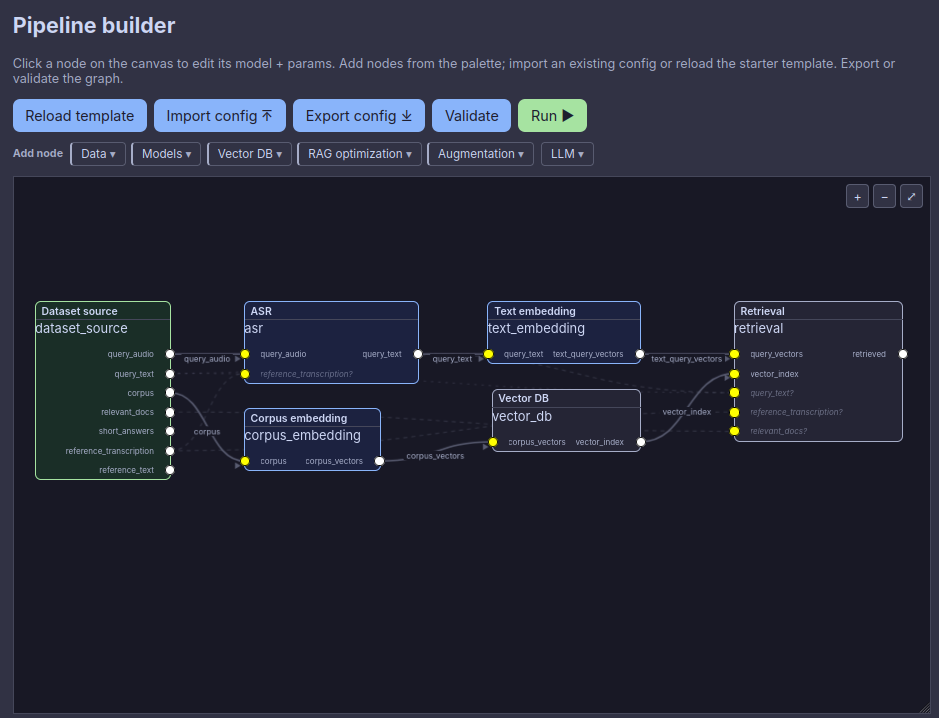
\includegraphics[width=0.92\linewidth]{figures/builder_ui.png}
    \caption{Edytor wizualny grafu. Gniazda węzłów opisane są nazwami artefaktów, a wejścia
    opcjonalne zaznaczono kursywą. Pokazany graf odpowiada ścieżce kaskadowej.}
    \label{fig:builderUi}
\end{figure}

\subsection{Ograniczenia i kod źródłowy}
\label{sec:ograniczenia}
Przyjęte założenia wyznaczają trzy granice zastosowania. Graf jest ustalony w chwili budowy, więc
sterowanie zależne od danych trzeba zamknąć w jednym węźle, którego wnętrze pozostaje
nieprzejrzyste dla proweniencji. Przebieg wykonywany jest w obrębie jednej maszyny, a większy
korpus obsługuje przetwarzanie oknami, nie rozdzielenie pracy między osobne węzły obliczeniowe.
Granicą pozostaje zatem pojemność jednej maszyny. Generacja odpowiedzi i sędzia korzystają z zewnętrznej
usługi modelu językowego, więc ich odtwarzalność jest względna wobec serwera, a jakość odpowiedzi
ocenia sędzia automatyczny wraz z heurystykami leksykalnymi, nie klinicysta.

Osobne ograniczenia wnosi sam zbiór badawczy. Ścieżka głosowa nie pochodzi z nagrań, lecz jest
syntezowana w czasie wykonania, więc nie obejmuje zmienności osobniczej mówcy, wad wymowy ani
zakłóceń otoczenia. Według wiedzy autorów nie istnieje też publiczny medyczny zbiór pytań i dokumentów w języku polskim
o strukturze wymaganej do oceny wyszukiwania, dlatego PubMedQA przetłumaczono na polski modelem
językowym. Tłumaczenie maszynowe wnosi własny błąd, uproszczenia terminologii i kalki składniowe,
który nakłada się na mierzone różnice między architekturami i którego niniejsza praca od nich nie
rozdziela. Zbiór polski jest przy tym mały, sto pytań i sto dokumentów; konsekwencje tej skali
dla zasięgu wniosków omówiono w podrozdziale~\ref{sec:jezyk}.

Implementację w języku Python udostępniono na licencji MIT wraz z konfiguracjami opisanych
eksperymentów \cite{reteva}.
